\documentclass{oblivoir}
\usepackage{amsmath,amssymb,amsthm,kotex,mdframed,paralist,chngcntr}
\usepackage{kswrapfig}

\newcounter{num}
%\newcommand{\defi}[1]
%{\bigskip\noindent\refstepcounter{num}\textbf{정의 \arabic{num}) #1}\par}
%\newcommand{\theo}[1]
%{\bigskip\noindent\refstepcounter{num}\textbf{정리 \arabic{num}) #1}\par}
%\newcommand{\exam}[1]
%{\bigskip\noindent\refstepcounter{num}\textbf{예시 \arabic{num}) #1}\par}
\newcommand{\prob}[1]
{\bigskip\noindent\refstepcounter{num}\textbf{문제 \arabic{num}) #1}\par}
%\newcommand{\howo}[1]
%{\bigskip\noindent\refstepcounter{num}\textbf{숙제 \arabic{num}) #1}\par\bigskip}

\newcommand{\ans}{{\raggedleft\textbf{답 : (\qquad\qquad\qquad\qquad\qquad\qquad)}
\par}}

\renewcommand{\proofname}{증명)}
\counterwithout{subsection}{section}


%%%
\begin{document}
\Large

\title{승재 04 - 최고수준 수학}
\author{}
\date{\today}
\maketitle
%\tableofcontents

\newpage

%
\prob{p103, \#05-1}
\kswrapfig[Pos=r]{103-05-1}{
오른쪽 그림은 한 변이 10cm인 정사각형 안에 반지름이 10cm인 원의 일부분 2개를 그린 것입니다.
A와 B의 넓이의 차를 구하세요.
(원주율 : 3)

\ans{}
}

%
\prob{p103, \#05-2}
아래 그림과 같이 \(A\)에서 \(B\)와 \(C\)를 거쳐 \(D\)로 가는 길이 있습니다.
길들은 모두 반원이며, 선분 \(AB\)의 길이는 \(400\)m이고, 선분 \(CD\)의 길이는 \(600\)m입니다.
철수는 \(A\)를 출발해 \(C\)까지 걸어가고 영희는 \(B\)를 출발해 \(D\)까지 걸어갑니다.
철수와 영희가 걷는 속력이 \(5\)m/s로 같을 때, 둘 중 누가 먼저 목적지에 도착하며, 도착시간의 차는 몇 초입니까?
(원주율 : 3.1)

\begin{figure}[h]
\centering
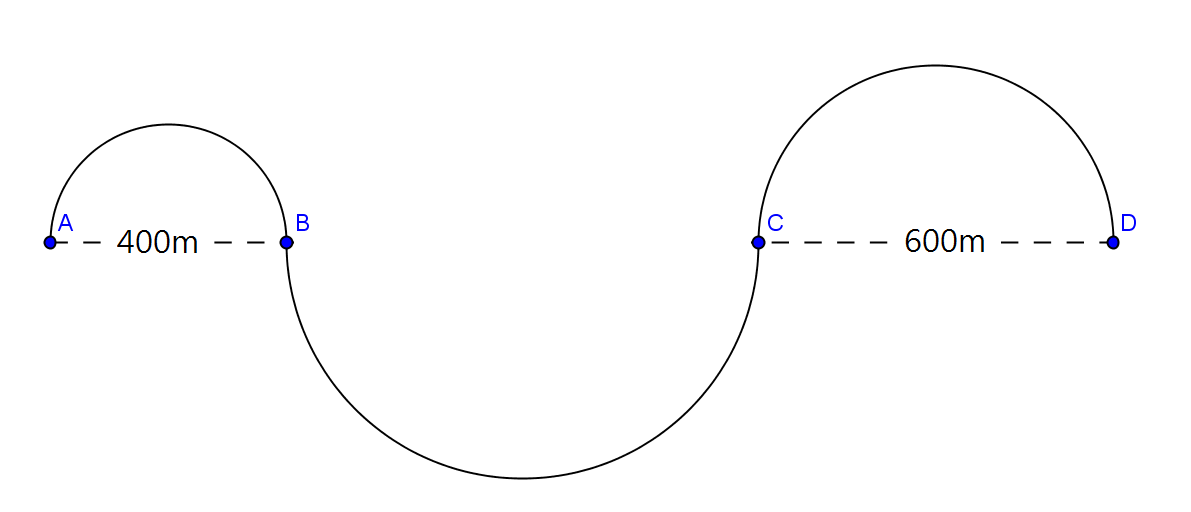
\includegraphics[width=0.7\textwidth]{103-05-2}
\end{figure}

{\raggedleft\textbf{답 : (\qquad\qquad\qquad)가 (\qquad\qquad\qquad)초 빨리 도착합니다.}
\par}

\newpage

%
\prob{p104, \#08-1}
\kswrapfig[Pos=r]{104-08-1}{
오른쪽 그림은 직각삼각형 안에 원을 꽉 차게 그린 것입니다.
원주를 구하여 소수 둘째자리에서 반올림하세요.
(원주율 : 3.14)

\ans{}
}

%
\prob{p104, \#08-2}
아래 그림과 같은 직각삼각형에서 사각형 ㅁㄴㅂㄹ는 정사각형입니다.
선분 ㅁㄹ의 길이를 구하세요.

\begin{figure}[h]
\centering
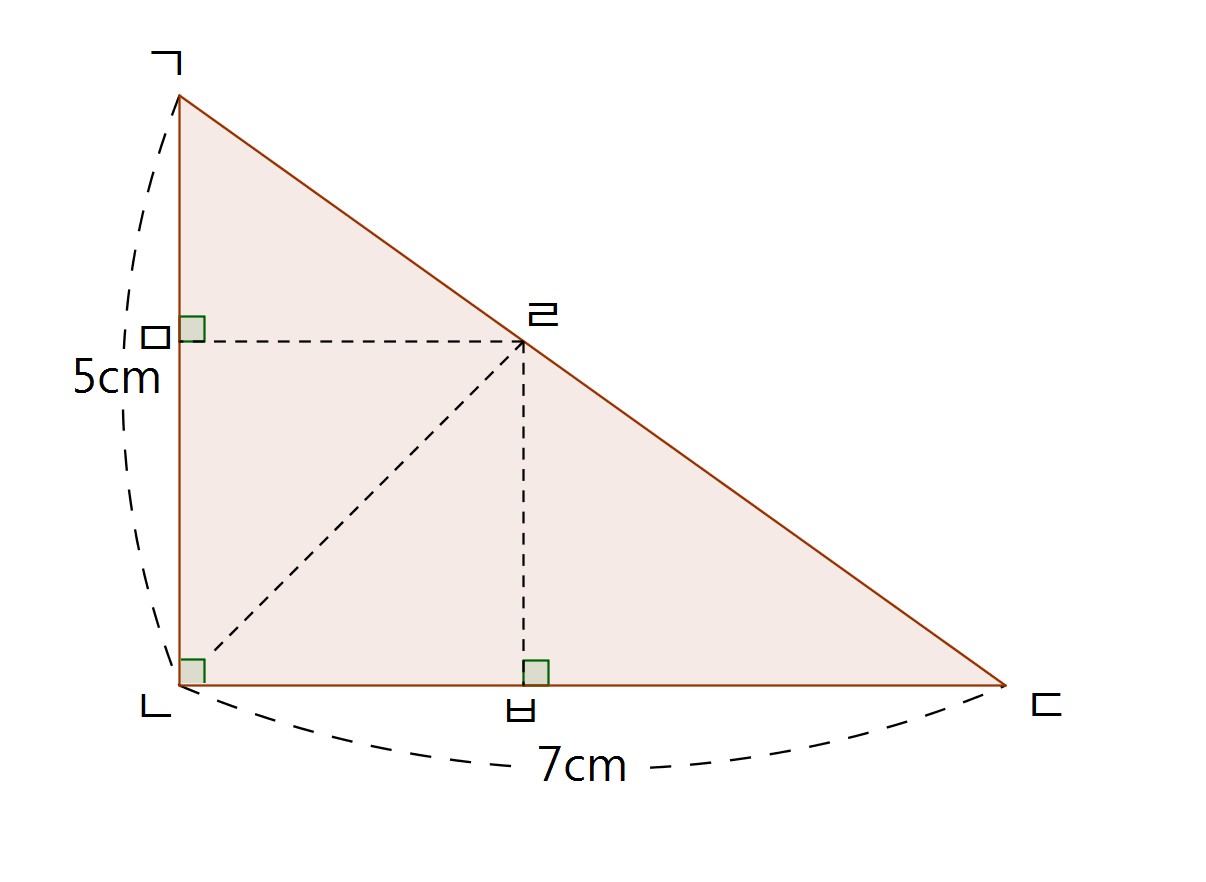
\includegraphics[width=0.7\textwidth]{104-08-2}
\end{figure}

\ans{}




\end{document}